% Generated by scripts/build_result_evidence.py. Requires longtable, graphicx, array.

% Parent manuscript controls appendix numbering and one-column placement.

\section{Archive-derived quantitative evidence}\label{sec:evidence-appendix}

\subsection{Observations, estimands, and pairing}

The root metrics files contain 98 completed R78 outputs and 70 completed R79 outputs. Each arm has seven tasks and two seeds (14 outputs). Cup/night uses seeds 10 and 17; every other task uses 0 and 17. The six source IDs are the clustering units. Dog/rain and dog/snow share source 121000000003 and remain together in every resample and sign flip. Historical sibling references in the archives are excluded from these counts.

Each contrast is first-listed arm minus second-listed arm, paired by task, seed, and source ID. All six contrasts have 14 complete pairs, seven tasks, six source clusters, and zero missing pairs. The CSV tables retain exact archive arm names, case IDs, recorded source PNG digests, and raw fields. Local NCC and whole-image source MAE are source-similarity measurements. The archive summaries record zero semantic judgments in both studies; no semantic scores are imputed.

Let $d_{cts}$ be a paired metric difference for source $c$, task $t$, and seed $s$, and let $\bar d_{ct}$ average the two seeds. The task-weighted estimate is $\sum_c\sum_{t\in c}\bar d_{ct}/7$. The source-weighted estimate is $\frac16\sum_c |T_c|^{-1}\sum_{t\in c}\bar d_{ct}$. Thus the dog source receives weight $2/7$ in the former and $1/6$ in the latter. All other sources receive $1/7$ and $1/6$, respectively.

Paired source-cluster bootstrap intervals use 100,000 draws of six source IDs with replacement, retaining every paired task and seed within a selected source. Each draw recomputes the stated estimand, including its task-count denominator. The 95\% intervals are percentile intervals with linear quantiles. NumPy PCG64 seed 20261030 is fixed, and identical cluster draws are reused across metrics and contrasts. Seeds are not resampled independently. These descriptive intervals summarize source-level variation in the six-source development set.

Exact two-sided source sign-flip values enumerate all $2^6=64$ assignments and compare absolute weighted mean differences with the observed absolute difference. They use a source-level sign-symmetry assumption and are reported as descriptive, unadjusted values. No confirmatory hypothesis family is declared; no Holm adjustment is applied. The smallest attainable nonzero two-sided value for six nonzero source effects is 0.03125.

\subsection{Selected descriptive contrasts}

\noindent\textbf{R78: ROUTE25 - U25\_KV.} All 14 task--seed pairs are matched in six source clusters.

\noindent\textbf{R78: ROI\_UNIFORM25 - ROUTE25.} All 14 task--seed pairs are matched in six source clusters.

\noindent\textbf{R78: ROUTE25 - ROUTE\_SHIFT25.} All 14 task--seed pairs are matched in six source clusters.

\begingroup\scriptsize\setlength{\tabcolsep}{2pt}
\begin{longtable}{p{.27\linewidth}p{.13\linewidth}lrrr}
\caption{R78 paired contrasts; differences are first arm minus second arm. All rows use 14 pairs and six source clusters. $p$ is the unadjusted exact source sign-flip value.}\\
\hline
Contrast & Metric & Weight & Difference & 95\% CI & $p$ \\ \hline
\endfirsthead
\hline
Contrast & Metric & Weight & Difference & 95\% CI & $p$ \\ \hline
\endhead
ROUTE25 - U25\_KV & NCC$_{\pm6}$ & Task & 0.1620 & [0.0959, 0.2441] & 0.03125 \\
ROUTE25 - U25\_KV & NCC$_{\pm6}$ & Source & 0.1788 & [0.1111, 0.2479] & 0.03125 \\
ROUTE25 - U25\_KV & Fixed NCC & Task & 0.1670 & [0.1046, 0.2463] & 0.03125 \\
ROUTE25 - U25\_KV & Fixed NCC & Source & 0.1831 & [0.1185, 0.2491] & 0.03125 \\
ROUTE25 - U25\_KV & Source MAE & Task & 0.0020 & [-0.0041, 0.0064] & 0.53125 \\
ROUTE25 - U25\_KV & Source MAE & Source & 0.0013 & [-0.0046, 0.0064] & 0.68750 \\
ROUTE25 - U25\_KV & Impulse $I$ & Task & -0.0000 & [-0.0000, 0.0000] & 0.78125 \\
ROUTE25 - U25\_KV & Impulse $I$ & Source & -0.0000 & [-0.0000, 0.0000] & 0.84375 \\
ROI\_UNIFORM25 - ROUTE25 & NCC$_{\pm6}$ & Task & 0.0975 & [0.0489, 0.1605] & 0.03125 \\
ROI\_UNIFORM25 - ROUTE25 & NCC$_{\pm6}$ & Source & 0.1104 & [0.0595, 0.1605] & 0.03125 \\
ROI\_UNIFORM25 - ROUTE25 & Fixed NCC & Task & 0.1010 & [0.0525, 0.1614] & 0.03125 \\
ROI\_UNIFORM25 - ROUTE25 & Fixed NCC & Source & 0.1143 & [0.0673, 0.1614] & 0.03125 \\
ROI\_UNIFORM25 - ROUTE25 & Source MAE & Task & 0.0481 & [0.0285, 0.0742] & 0.03125 \\
ROI\_UNIFORM25 - ROUTE25 & Source MAE & Source & 0.0508 & [0.0275, 0.0743] & 0.03125 \\
ROI\_UNIFORM25 - ROUTE25 & Impulse $I$ & Task & 0.0000 & [-0.0000, 0.0000] & 0.59375 \\
ROI\_UNIFORM25 - ROUTE25 & Impulse $I$ & Source & 0.0000 & [-0.0000, 0.0000] & 0.68750 \\
ROUTE25 - ROUTE\_SHIFT25 & NCC$_{\pm6}$ & Task & 0.2423 & [0.1619, 0.3444] & 0.03125 \\
ROUTE25 - ROUTE\_SHIFT25 & NCC$_{\pm6}$ & Source & 0.2628 & [0.1795, 0.3461] & 0.03125 \\
ROUTE25 - ROUTE\_SHIFT25 & Fixed NCC & Task & 0.2546 & [0.1758, 0.3544] & 0.03125 \\
ROUTE25 - ROUTE\_SHIFT25 & Fixed NCC & Source & 0.2740 & [0.1932, 0.3571] & 0.03125 \\
ROUTE25 - ROUTE\_SHIFT25 & Source MAE & Task & 0.0019 & [-0.0004, 0.0054] & 0.25000 \\
ROUTE25 - ROUTE\_SHIFT25 & Source MAE & Source & 0.0025 & [0.0000, 0.0055] & 0.15625 \\
ROUTE25 - ROUTE\_SHIFT25 & Impulse $I$ & Task & -0.0000 & [-0.0000, 0.0000] & 0.93750 \\
ROUTE25 - ROUTE\_SHIFT25 & Impulse $I$ & Source & -0.0000 & [-0.0000, 0.0000] & 0.93750 \\
\hline\end{longtable}
\endgroup

\noindent\textbf{R79: ROI\_ONLINE25 - ROI\_LOCAL25.} All 14 task--seed pairs are matched in six source clusters.

\noindent\textbf{R79: ROI\_ONLINE25\_QROI - ROI\_ONLINE25.} All 14 task--seed pairs are matched in six source clusters.

\noindent\textbf{R79: ROI\_LOCAL25 - ROI\_LOCAL25\_OFF.} All 14 task--seed pairs are matched in six source clusters.

\begingroup\scriptsize\setlength{\tabcolsep}{2pt}
\begin{longtable}{p{.27\linewidth}p{.13\linewidth}lrrr}
\caption{R79 paired contrasts; differences are first arm minus second arm. All rows use 14 pairs and six source clusters. $p$ is the unadjusted exact source sign-flip value.}\\
\hline
Contrast & Metric & Weight & Difference & 95\% CI & $p$ \\ \hline
\endfirsthead
\hline
Contrast & Metric & Weight & Difference & 95\% CI & $p$ \\ \hline
\endhead
ROI\_ONLINE25 - ROI\_LOCAL25 & NCC$_{\pm6}$ & Task & 0.3420 & [0.2238, 0.4824] & 0.03125 \\
ROI\_ONLINE25 - ROI\_LOCAL25 & NCC$_{\pm6}$ & Source & 0.3725 & [0.2518, 0.4824] & 0.03125 \\
ROI\_ONLINE25 - ROI\_LOCAL25 & Fixed NCC & Task & 0.3538 & [0.2445, 0.4872] & 0.03125 \\
ROI\_ONLINE25 - ROI\_LOCAL25 & Fixed NCC & Source & 0.3816 & [0.2686, 0.4872] & 0.03125 \\
ROI\_ONLINE25 - ROI\_LOCAL25 & Source MAE & Task & -0.0103 & [-0.0133, -0.0061] & 0.03125 \\
ROI\_ONLINE25 - ROI\_LOCAL25 & Source MAE & Source & -0.0096 & [-0.0130, -0.0061] & 0.03125 \\
ROI\_ONLINE25 - ROI\_LOCAL25 & Impulse $I$ & Task & 0.1604 & [0.1398, 0.1846] & 0.03125 \\
ROI\_ONLINE25 - ROI\_LOCAL25 & Impulse $I$ & Source & 0.1632 & [0.1391, 0.1860] & 0.03125 \\
ROI\_ONLINE25\_QROI - ROI\_ONLINE25 & NCC$_{\pm6}$ & Task & -0.0272 & [-0.0901, 0.0210] & 0.50000 \\
ROI\_ONLINE25\_QROI - ROI\_ONLINE25 & NCC$_{\pm6}$ & Source & -0.0325 & [-0.0945, 0.0243] & 0.50000 \\
ROI\_ONLINE25\_QROI - ROI\_ONLINE25 & Fixed NCC & Task & -0.0319 & [-0.1062, 0.0215] & 0.50000 \\
ROI\_ONLINE25\_QROI - ROI\_ONLINE25 & Fixed NCC & Source & -0.0381 & [-0.1114, 0.0246] & 0.50000 \\
ROI\_ONLINE25\_QROI - ROI\_ONLINE25 & Source MAE & Task & 0.0807 & [0.0449, 0.1104] & 0.03125 \\
ROI\_ONLINE25\_QROI - ROI\_ONLINE25 & Source MAE & Source & 0.0725 & [0.0449, 0.1013] & 0.03125 \\
ROI\_ONLINE25\_QROI - ROI\_ONLINE25 & Impulse $I$ & Task & 0.0522 & [0.0284, 0.0706] & 0.03125 \\
ROI\_ONLINE25\_QROI - ROI\_ONLINE25 & Impulse $I$ & Source & 0.0481 & [0.0284, 0.0680] & 0.03125 \\
ROI\_LOCAL25 - ROI\_LOCAL25\_OFF & NCC$_{\pm6}$ & Task & 0.2770 & [0.1029, 0.4098] & 0.06250 \\
ROI\_LOCAL25 - ROI\_LOCAL25\_OFF & NCC$_{\pm6}$ & Source & 0.2486 & [0.1000, 0.3972] & 0.06250 \\
ROI\_LOCAL25 - ROI\_LOCAL25\_OFF & Fixed NCC & Task & 0.2841 & [0.1103, 0.4165] & 0.06250 \\
ROI\_LOCAL25 - ROI\_LOCAL25\_OFF & Fixed NCC & Source & 0.2578 & [0.1076, 0.4080] & 0.06250 \\
ROI\_LOCAL25 - ROI\_LOCAL25\_OFF & Source MAE & Task & -0.0927 & [-0.1268, -0.0530] & 0.03125 \\
ROI\_LOCAL25 - ROI\_LOCAL25\_OFF & Source MAE & Source & -0.0828 & [-0.1149, -0.0530] & 0.03125 \\
ROI\_LOCAL25 - ROI\_LOCAL25\_OFF & Impulse $I$ & Task & -0.0094 & [-0.0113, -0.0072] & 0.03125 \\
ROI\_LOCAL25 - ROI\_LOCAL25\_OFF & Impulse $I$ & Source & -0.0089 & [-0.0106, -0.0072] & 0.03125 \\
\hline\end{longtable}
\endgroup

\begin{figure}[htbp]\centering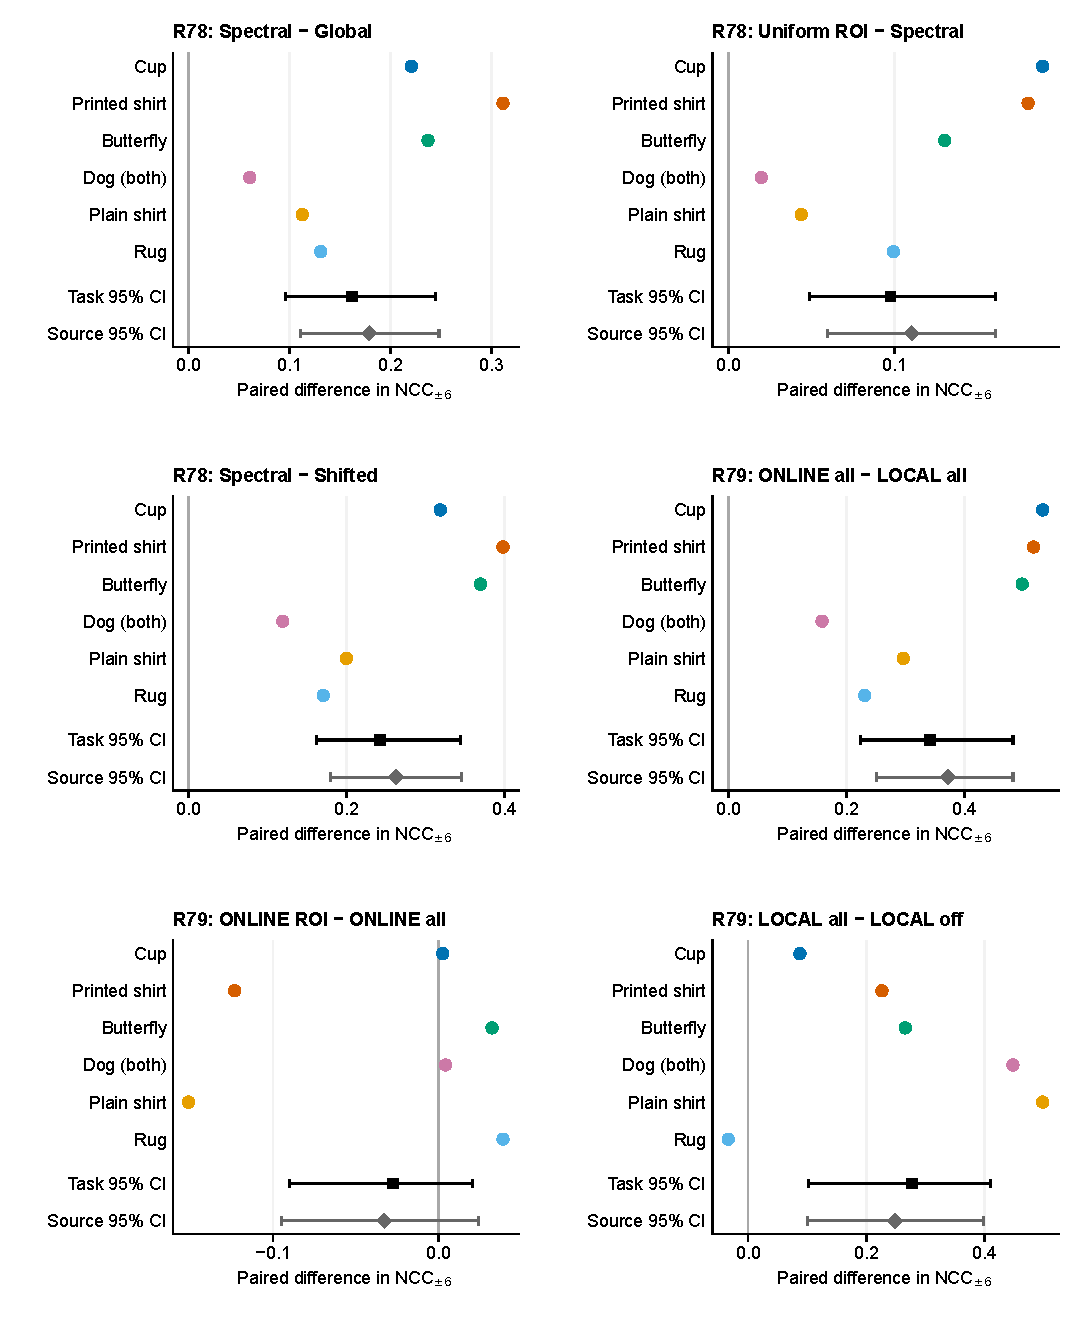
\includegraphics[width=\linewidth]{figures/evidence_paired_ncc.pdf}\caption{Source-level paired differences in shift-tolerant local NCC. Each colored point averages seeds and, for dog, both tasks. Squares and diamonds show task-weighted and source-weighted estimates with paired source-cluster bootstrap 95\% intervals. Differences follow the panel titles.}\label{fig:evidence-paired_ncc}\end{figure}

\begin{figure}[htbp]\centering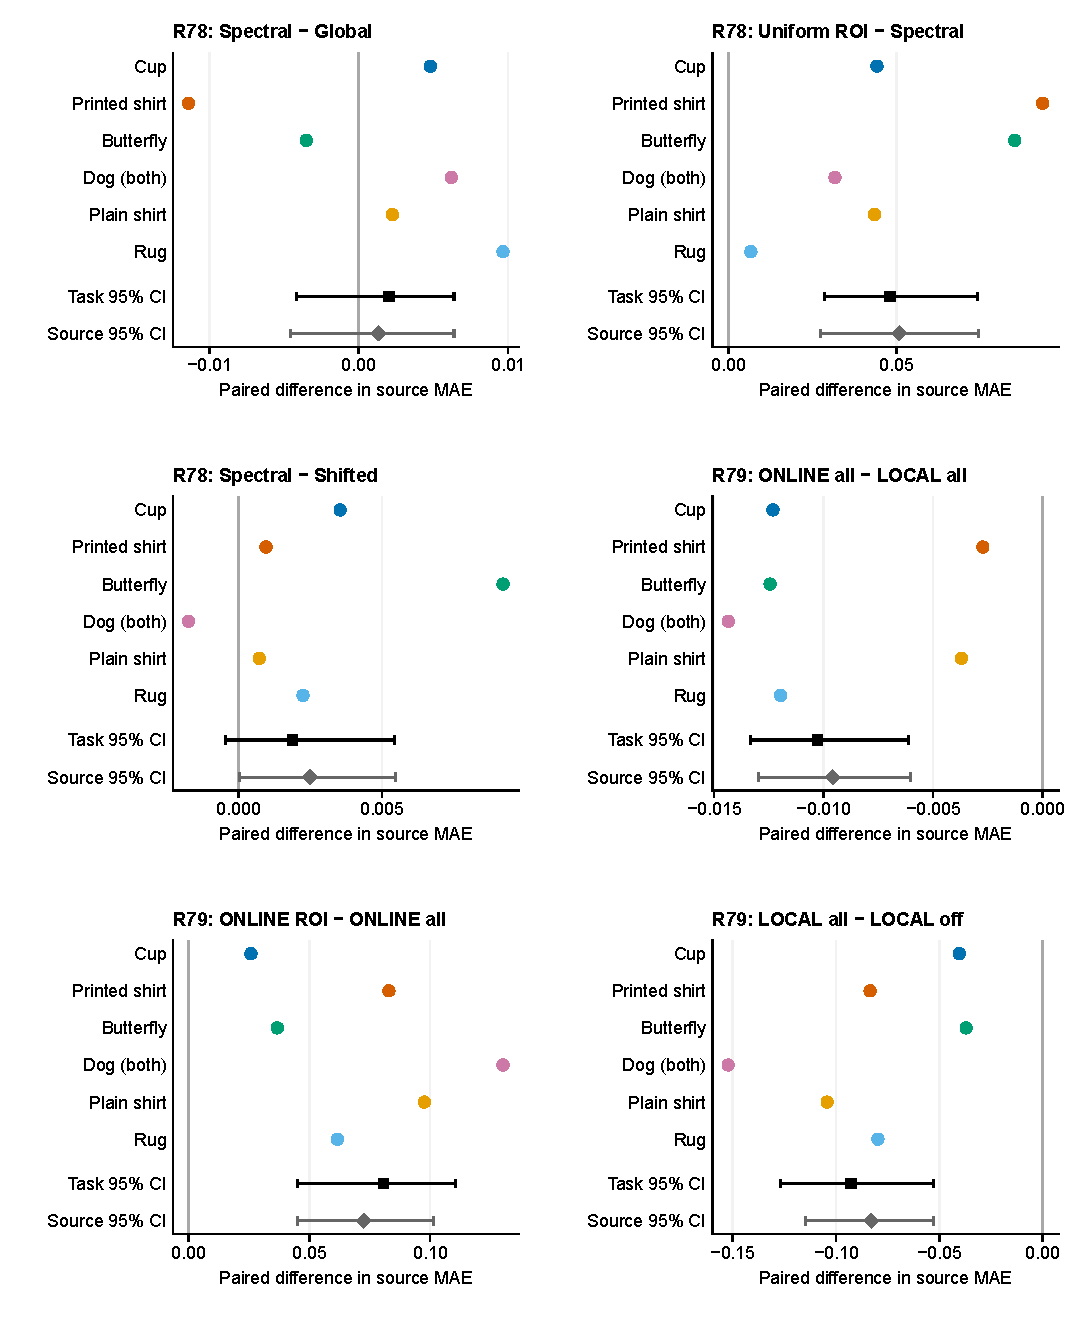
\includegraphics[width=\linewidth]{figures/evidence_paired_mae.pdf}\caption{Source-level paired differences in whole-image source MAE, with the same pairing and weights as the NCC plot. A positive difference means greater departure from the source image.}\label{fig:evidence-paired_mae}\end{figure}

\begin{figure}[htbp]\centering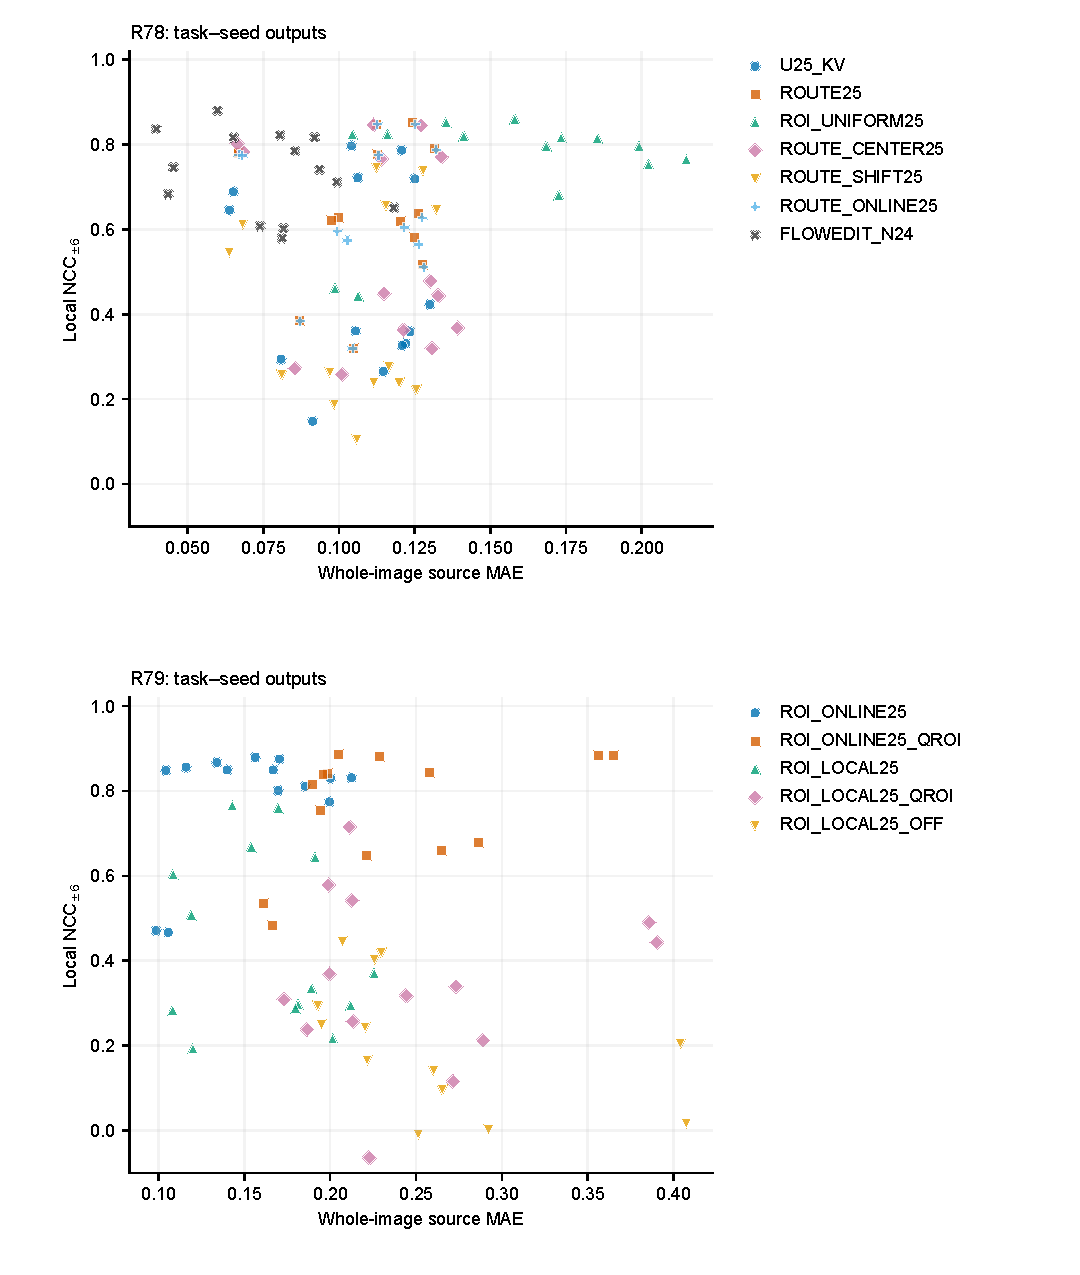
\includegraphics[width=\linewidth]{figures/evidence_ncc_source_mae_scatter.pdf}\caption{Local NCC versus whole-image source MAE for every completed task--seed output (98 R78, 70 R79). Colors and markers identify the recorded arms. Outputs sharing sources are dependent; these axes describe source correlation and source departure.}\label{fig:evidence-ncc_source_mae_scatter}\end{figure}

\subsection{Complete task-by-arm means and seed-level results}

Task codes: C = cup\_night; P = printed\_shirt\_studio; B = butterfly\_sunset; DS = dog\_snow; DR = dog\_rain; S = shirt\_studio; R = rug\_floor. Each task-by-arm row averages exactly two seeds. $I$ is the logged integrated correction impulse; a dash denotes an unavailable value. CSV exports retain the full precision and all original metric fields.

\begingroup\scriptsize\setlength{\tabcolsep}{2pt}
\begin{longtable}{lp{.29\linewidth}lrrrr}
\caption{All-arm aggregate means under both weighting rules. Each arm has 14 outputs, seven tasks, and six source clusters.}\\
\hline
Study & Arm & Weight & MAE & Fixed NCC & NCC$_{\pm6}$ & $I$ \\ \hline
\endfirsthead
\hline
Study & Arm & Weight & MAE & Fixed NCC & NCC$_{\pm6}$ & $I$ \\ \hline
\endhead
R78 & U25\_KV & Task & 0.1053 & 0.4799 & 0.4901 & 0.2260 \\
R78 & U25\_KV & Source & 0.1038 & 0.4365 & 0.4459 & 0.2258 \\
R78 & ROUTE25 & Task & 0.1073 & 0.6469 & 0.6521 & 0.2260 \\
R78 & ROUTE25 & Source & 0.1052 & 0.6196 & 0.6247 & 0.2258 \\
R78 & ROI\_UNIFORM25 & Task & 0.1554 & 0.7479 & 0.7496 & 0.2260 \\
R78 & ROI\_UNIFORM25 & Source & 0.1560 & 0.7339 & 0.7352 & 0.2258 \\
R78 & ROUTE\_CENTER25 & Task & 0.1126 & 0.5506 & 0.5542 & 0.2260 \\
R78 & ROUTE\_CENTER25 & Source & 0.1111 & 0.5092 & 0.5121 & 0.2258 \\
R78 & ROUTE\_SHIFT25 & Task & 0.1054 & 0.3923 & 0.4098 & 0.2260 \\
R78 & ROUTE\_SHIFT25 & Source & 0.1027 & 0.3456 & 0.3619 & 0.2258 \\
R78 & ROUTE\_ONLINE25 & Task & 0.1083 & 0.6369 & 0.6416 & 0.2221 \\
R78 & ROUTE\_ONLINE25 & Source & 0.1062 & 0.6084 & 0.6129 & 0.2217 \\
R78 & FLOWEDIT\_N24 & Task & 0.0757 & 0.7322 & 0.7339 & -- \\
R78 & FLOWEDIT\_N24 & Source & 0.0734 & 0.7245 & 0.7256 & -- \\
R79 & ROI\_ONLINE25 & Task & 0.1543 & 0.7857 & 0.7864 & 0.2524 \\
R79 & ROI\_ONLINE25 & Source & 0.1549 & 0.7722 & 0.7729 & 0.2513 \\
R79 & ROI\_ONLINE25\_QROI & Task & 0.2350 & 0.7538 & 0.7592 & 0.3046 \\
R79 & ROI\_ONLINE25\_QROI & Source & 0.2274 & 0.7341 & 0.7403 & 0.2994 \\
R79 & ROI\_LOCAL25 & Task & 0.1645 & 0.4319 & 0.4445 & 0.0921 \\
R79 & ROI\_LOCAL25 & Source & 0.1645 & 0.3906 & 0.4004 & 0.0881 \\
R79 & ROI\_LOCAL25\_QROI & Task & 0.2481 & 0.3164 & 0.3473 & 0.0945 \\
R79 & ROI\_LOCAL25\_QROI & Source & 0.2394 & 0.2835 & 0.3140 & 0.0900 \\
R79 & ROI\_LOCAL25\_OFF & Task & 0.2573 & 0.1478 & 0.1674 & 0.1015 \\
R79 & ROI\_LOCAL25\_OFF & Source & 0.2474 & 0.1327 & 0.1518 & 0.0970 \\
\hline\end{longtable}
\endgroup

\begingroup\scriptsize\setlength{\tabcolsep}{2pt}
\begin{longtable}{lp{.30\linewidth}rrrr}
\caption{R78 complete task-by-arm means ($n=2$ seeds each).}\\
\hline
Task & Recorded arm & MAE & Fixed NCC & NCC$_{\pm6}$ & $I$ \\ \hline
\endfirsthead
\hline
Task & Recorded arm & MAE & Fixed NCC & NCC$_{\pm6}$ & $I$ \\ \hline
\endhead
C & U25\_KV & 0.1215 & 0.3284 & 0.3284 & 0.2414 \\
C & ROUTE25 & 0.1263 & 0.5489 & 0.5489 & 0.2414 \\
C & ROI\_UNIFORM25 & 0.1705 & 0.7380 & 0.7380 & 0.2414 \\
C & ROUTE\_CENTER25 & 0.1316 & 0.4605 & 0.4605 & 0.2414 \\
C & ROUTE\_SHIFT25 & 0.1227 & 0.2217 & 0.2301 & 0.2414 \\
C & ROUTE\_ONLINE25 & 0.1273 & 0.5375 & 0.5375 & 0.2379 \\
C & FLOWEDIT\_N24 & 0.1059 & 0.6960 & 0.6960 & -- \\
P & U25\_KV & 0.1101 & 0.3118 & 0.3127 & 0.2262 \\
P & ROUTE25 & 0.0987 & 0.6240 & 0.6240 & 0.2262 \\
P & ROI\_UNIFORM25 & 0.1923 & 0.8043 & 0.8043 & 0.2262 \\
P & ROUTE\_CENTER25 & 0.1181 & 0.4059 & 0.4059 & 0.2262 \\
P & ROUTE\_SHIFT25 & 0.0978 & 0.2185 & 0.2257 & 0.2262 \\
P & ROUTE\_ONLINE25 & 0.1011 & 0.5844 & 0.5844 & 0.2165 \\
P & FLOWEDIT\_N24 & 0.0695 & 0.7121 & 0.7121 & -- \\
B & U25\_KV & 0.1268 & 0.3907 & 0.3907 & 0.2387 \\
B & ROUTE25 & 0.1232 & 0.6278 & 0.6278 & 0.2387 \\
B & ROI\_UNIFORM25 & 0.2085 & 0.7579 & 0.7579 & 0.2387 \\
B & ROUTE\_CENTER25 & 0.1349 & 0.3428 & 0.3428 & 0.2387 \\
B & ROUTE\_SHIFT25 & 0.1140 & 0.2383 & 0.2579 & 0.2387 \\
B & ROUTE\_ONLINE25 & 0.1245 & 0.6155 & 0.6155 & 0.2332 \\
B & FLOWEDIT\_N24 & 0.0815 & 0.5904 & 0.5904 & -- \\
DS & U25\_KV & 0.1229 & 0.7354 & 0.7526 & 0.2285 \\
DS & ROUTE25 & 0.1279 & 0.8135 & 0.8213 & 0.2285 \\
DS & ROI\_UNIFORM25 & 0.1657 & 0.8321 & 0.8373 & 0.2285 \\
DS & ROUTE\_CENTER25 & 0.1305 & 0.7982 & 0.8075 & 0.2285 \\
DS & ROUTE\_SHIFT25 & 0.1300 & 0.6662 & 0.6927 & 0.2285 \\
DS & ROUTE\_ONLINE25 & 0.1286 & 0.8092 & 0.8172 & 0.2256 \\
DS & FLOWEDIT\_N24 & 0.0956 & 0.7537 & 0.7634 & -- \\
DR & U25\_KV & 0.1052 & 0.7459 & 0.7589 & 0.2253 \\
DR & ROUTE25 & 0.1127 & 0.8078 & 0.8117 & 0.2253 \\
DR & ROI\_UNIFORM25 & 0.1383 & 0.8314 & 0.8355 & 0.2253 \\
DR & ROUTE\_CENTER25 & 0.1127 & 0.8009 & 0.8056 & 0.2253 \\
DR & ROUTE\_SHIFT25 & 0.1140 & 0.6795 & 0.7014 & 0.2253 \\
DR & ROUTE\_ONLINE25 & 0.1129 & 0.8068 & 0.8108 & 0.2238 \\
DR & FLOWEDIT\_N24 & 0.0829 & 0.8025 & 0.8032 & -- \\
S & U25\_KV & 0.0645 & 0.6375 & 0.6667 & 0.2144 \\
S & ROUTE25 & 0.0667 & 0.7544 & 0.7792 & 0.2144 \\
S & ROI\_UNIFORM25 & 0.1102 & 0.8203 & 0.8231 & 0.2144 \\
S & ROUTE\_CENTER25 & 0.0675 & 0.7859 & 0.7920 & 0.2144 \\
S & ROUTE\_SHIFT25 & 0.0660 & 0.5452 & 0.5793 & 0.2144 \\
S & ROUTE\_ONLINE25 & 0.0675 & 0.7535 & 0.7745 & 0.2111 \\
S & FLOWEDIT\_N24 & 0.0498 & 0.8568 & 0.8581 & -- \\
R & U25\_KV & 0.0861 & 0.2097 & 0.2209 & 0.2074 \\
R & ROUTE25 & 0.0958 & 0.3519 & 0.3519 & 0.2074 \\
R & ROI\_UNIFORM25 & 0.1025 & 0.4512 & 0.4512 & 0.2074 \\
R & ROUTE\_CENTER25 & 0.0932 & 0.2601 & 0.2648 & 0.2074 \\
R & ROUTE\_SHIFT25 & 0.0935 & 0.1768 & 0.1814 & 0.2074 \\
R & ROUTE\_ONLINE25 & 0.0959 & 0.3515 & 0.3515 & 0.2065 \\
R & FLOWEDIT\_N24 & 0.0445 & 0.7139 & 0.7139 & -- \\
\hline\end{longtable}
\endgroup

\begingroup\scriptsize\setlength{\tabcolsep}{2pt}
\begin{longtable}{llp{.29\linewidth}rrrr}
\caption{R78 complete per-seed quantitative results.}\\
\hline
Task & Seed & Recorded arm & MAE & Fixed NCC & NCC$_{\pm6}$ & $I$ \\ \hline
\endfirsthead
\hline
Task & Seed & Recorded arm & MAE & Fixed NCC & NCC$_{\pm6}$ & $I$ \\ \hline
\endhead
C & 10 & U25\_KV & 0.1220 & 0.3307 & 0.3307 & 0.2422 \\
C & 17 & U25\_KV & 0.1209 & 0.3261 & 0.3261 & 0.2406 \\
C & 10 & ROUTE25 & 0.1250 & 0.5799 & 0.5799 & 0.2422 \\
C & 17 & ROUTE25 & 0.1275 & 0.5180 & 0.5180 & 0.2406 \\
C & 10 & ROI\_UNIFORM25 & 0.1684 & 0.7957 & 0.7957 & 0.2422 \\
C & 17 & ROI\_UNIFORM25 & 0.1726 & 0.6803 & 0.6803 & 0.2406 \\
C & 10 & ROUTE\_CENTER25 & 0.1328 & 0.4432 & 0.4432 & 0.2422 \\
C & 17 & ROUTE\_CENTER25 & 0.1303 & 0.4778 & 0.4778 & 0.2406 \\
C & 10 & ROUTE\_SHIFT25 & 0.1199 & 0.2339 & 0.2381 & 0.2422 \\
C & 17 & ROUTE\_SHIFT25 & 0.1255 & 0.2094 & 0.2221 & 0.2406 \\
C & 10 & ROUTE\_ONLINE25 & 0.1264 & 0.5642 & 0.5642 & 0.2376 \\
C & 17 & ROUTE\_ONLINE25 & 0.1281 & 0.5108 & 0.5108 & 0.2382 \\
C & 10 & FLOWEDIT\_N24 & 0.1181 & 0.6503 & 0.6503 & -- \\
C & 17 & FLOWEDIT\_N24 & 0.0936 & 0.7416 & 0.7416 & -- \\
P & 0 & U25\_KV & 0.1147 & 0.2651 & 0.2651 & 0.2280 \\
P & 17 & U25\_KV & 0.1055 & 0.3586 & 0.3604 & 0.2245 \\
P & 0 & ROUTE25 & 0.0998 & 0.6279 & 0.6279 & 0.2280 \\
P & 17 & ROUTE25 & 0.0977 & 0.6201 & 0.6201 & 0.2245 \\
P & 0 & ROI\_UNIFORM25 & 0.1991 & 0.7947 & 0.7947 & 0.2280 \\
P & 17 & ROI\_UNIFORM25 & 0.1854 & 0.8139 & 0.8139 & 0.2245 \\
P & 0 & ROUTE\_CENTER25 & 0.1213 & 0.3623 & 0.3623 & 0.2280 \\
P & 17 & ROUTE\_CENTER25 & 0.1149 & 0.4495 & 0.4495 & 0.2245 \\
P & 0 & ROUTE\_SHIFT25 & 0.0985 & 0.1761 & 0.1879 & 0.2280 \\
P & 17 & ROUTE\_SHIFT25 & 0.0970 & 0.2609 & 0.2634 & 0.2245 \\
P & 0 & ROUTE\_ONLINE25 & 0.1029 & 0.5735 & 0.5735 & 0.2167 \\
P & 17 & ROUTE\_ONLINE25 & 0.0994 & 0.5953 & 0.5953 & 0.2164 \\
P & 0 & FLOWEDIT\_N24 & 0.0651 & 0.8168 & 0.8168 & -- \\
P & 17 & FLOWEDIT\_N24 & 0.0740 & 0.6074 & 0.6074 & -- \\
B & 0 & U25\_KV & 0.1300 & 0.4229 & 0.4229 & 0.2425 \\
B & 17 & U25\_KV & 0.1235 & 0.3585 & 0.3585 & 0.2348 \\
B & 0 & ROUTE25 & 0.1262 & 0.6380 & 0.6380 & 0.2425 \\
B & 17 & ROUTE25 & 0.1203 & 0.6175 & 0.6175 & 0.2348 \\
B & 0 & ROI\_UNIFORM25 & 0.2147 & 0.7638 & 0.7638 & 0.2425 \\
B & 17 & ROI\_UNIFORM25 & 0.2022 & 0.7520 & 0.7520 & 0.2348 \\
B & 0 & ROUTE\_CENTER25 & 0.1390 & 0.3675 & 0.3675 & 0.2425 \\
B & 17 & ROUTE\_CENTER25 & 0.1308 & 0.3182 & 0.3182 & 0.2348 \\
B & 0 & ROUTE\_SHIFT25 & 0.1165 & 0.2755 & 0.2766 & 0.2425 \\
B & 17 & ROUTE\_SHIFT25 & 0.1115 & 0.2012 & 0.2392 & 0.2348 \\
B & 0 & ROUTE\_ONLINE25 & 0.1275 & 0.6272 & 0.6272 & 0.2372 \\
B & 17 & ROUTE\_ONLINE25 & 0.1215 & 0.6039 & 0.6039 & 0.2293 \\
B & 0 & FLOWEDIT\_N24 & 0.0813 & 0.5793 & 0.5793 & -- \\
B & 17 & FLOWEDIT\_N24 & 0.0817 & 0.6015 & 0.6015 & -- \\
DS & 0 & U25\_KV & 0.1208 & 0.7829 & 0.7865 & 0.2285 \\
DS & 17 & U25\_KV & 0.1251 & 0.6880 & 0.7188 & 0.2285 \\
DS & 0 & ROUTE25 & 0.1243 & 0.8510 & 0.8520 & 0.2285 \\
DS & 17 & ROUTE25 & 0.1314 & 0.7760 & 0.7907 & 0.2285 \\
DS & 0 & ROI\_UNIFORM25 & 0.1581 & 0.8579 & 0.8594 & 0.2285 \\
DS & 17 & ROI\_UNIFORM25 & 0.1734 & 0.8064 & 0.8151 & 0.2285 \\
DS & 0 & ROUTE\_CENTER25 & 0.1271 & 0.8427 & 0.8445 & 0.2285 \\
DS & 17 & ROUTE\_CENTER25 & 0.1338 & 0.7537 & 0.7706 & 0.2285 \\
DS & 0 & ROUTE\_SHIFT25 & 0.1278 & 0.7312 & 0.7387 & 0.2285 \\
DS & 17 & ROUTE\_SHIFT25 & 0.1322 & 0.6013 & 0.6467 & 0.2285 \\
DS & 0 & ROUTE\_ONLINE25 & 0.1252 & 0.8459 & 0.8474 & 0.2246 \\
DS & 17 & ROUTE\_ONLINE25 & 0.1321 & 0.7726 & 0.7871 & 0.2267 \\
DS & 0 & FLOWEDIT\_N24 & 0.0993 & 0.6919 & 0.7111 & -- \\
DS & 17 & FLOWEDIT\_N24 & 0.0919 & 0.8156 & 0.8156 & -- \\
DR & 0 & U25\_KV & 0.1041 & 0.7929 & 0.7964 & 0.2254 \\
DR & 17 & U25\_KV & 0.1063 & 0.6989 & 0.7215 & 0.2253 \\
DR & 0 & ROUTE25 & 0.1124 & 0.8456 & 0.8477 & 0.2254 \\
DR & 17 & ROUTE25 & 0.1129 & 0.7701 & 0.7756 & 0.2253 \\
DR & 0 & ROI\_UNIFORM25 & 0.1354 & 0.8496 & 0.8516 & 0.2254 \\
DR & 17 & ROI\_UNIFORM25 & 0.1412 & 0.8133 & 0.8194 & 0.2253 \\
DR & 0 & ROUTE\_CENTER25 & 0.1114 & 0.8442 & 0.8460 & 0.2254 \\
DR & 17 & ROUTE\_CENTER25 & 0.1140 & 0.7576 & 0.7653 & 0.2253 \\
DR & 0 & ROUTE\_SHIFT25 & 0.1124 & 0.7378 & 0.7461 & 0.2254 \\
DR & 17 & ROUTE\_SHIFT25 & 0.1155 & 0.6212 & 0.6567 & 0.2253 \\
DR & 0 & ROUTE\_ONLINE25 & 0.1126 & 0.8452 & 0.8474 & 0.2242 \\
DR & 17 & ROUTE\_ONLINE25 & 0.1131 & 0.7684 & 0.7743 & 0.2234 \\
DR & 0 & FLOWEDIT\_N24 & 0.0854 & 0.7830 & 0.7844 & -- \\
DR & 17 & FLOWEDIT\_N24 & 0.0805 & 0.8220 & 0.8220 & -- \\
S & 0 & U25\_KV & 0.0638 & 0.6269 & 0.6451 & 0.2134 \\
S & 17 & U25\_KV & 0.0651 & 0.6481 & 0.6883 & 0.2154 \\
S & 0 & ROUTE25 & 0.0667 & 0.7781 & 0.7781 & 0.2134 \\
S & 17 & ROUTE25 & 0.0668 & 0.7306 & 0.7803 & 0.2154 \\
S & 0 & ROI\_UNIFORM25 & 0.1161 & 0.8226 & 0.8226 & 0.2134 \\
S & 17 & ROI\_UNIFORM25 & 0.1044 & 0.8180 & 0.8236 & 0.2154 \\
S & 0 & ROUTE\_CENTER25 & 0.0664 & 0.7978 & 0.8017 & 0.2134 \\
S & 17 & ROUTE\_CENTER25 & 0.0686 & 0.7741 & 0.7823 & 0.2154 \\
S & 0 & ROUTE\_SHIFT25 & 0.0638 & 0.5244 & 0.5464 & 0.2134 \\
S & 17 & ROUTE\_SHIFT25 & 0.0682 & 0.5659 & 0.6123 & 0.2154 \\
S & 0 & ROUTE\_ONLINE25 & 0.0670 & 0.7754 & 0.7754 & 0.2114 \\
S & 17 & ROUTE\_ONLINE25 & 0.0681 & 0.7317 & 0.7737 & 0.2109 \\
S & 0 & FLOWEDIT\_N24 & 0.0396 & 0.8355 & 0.8362 & -- \\
S & 17 & FLOWEDIT\_N24 & 0.0599 & 0.8781 & 0.8800 & -- \\
R & 0 & U25\_KV & 0.0809 & 0.2716 & 0.2939 & 0.2055 \\
R & 17 & U25\_KV & 0.0913 & 0.1479 & 0.1479 & 0.2094 \\
R & 0 & ROUTE25 & 0.0869 & 0.3853 & 0.3853 & 0.2055 \\
R & 17 & ROUTE25 & 0.1047 & 0.3184 & 0.3184 & 0.2094 \\
R & 0 & ROI\_UNIFORM25 & 0.0987 & 0.4598 & 0.4598 & 0.2055 \\
R & 17 & ROI\_UNIFORM25 & 0.1063 & 0.4426 & 0.4426 & 0.2094 \\
R & 0 & ROUTE\_CENTER25 & 0.0854 & 0.2624 & 0.2718 & 0.2055 \\
R & 17 & ROUTE\_CENTER25 & 0.1010 & 0.2578 & 0.2578 & 0.2094 \\
R & 0 & ROUTE\_SHIFT25 & 0.0811 & 0.2562 & 0.2568 & 0.2055 \\
R & 17 & ROUTE\_SHIFT25 & 0.1059 & 0.0974 & 0.1059 & 0.2094 \\
R & 0 & ROUTE\_ONLINE25 & 0.0872 & 0.3838 & 0.3838 & 0.2035 \\
R & 17 & ROUTE\_ONLINE25 & 0.1046 & 0.3191 & 0.3191 & 0.2096 \\
R & 0 & FLOWEDIT\_N24 & 0.0436 & 0.6823 & 0.6823 & -- \\
R & 17 & FLOWEDIT\_N24 & 0.0454 & 0.7454 & 0.7454 & -- \\
\hline\end{longtable}
\endgroup

\begingroup\scriptsize\setlength{\tabcolsep}{2pt}
\begin{longtable}{lp{.30\linewidth}rrrr}
\caption{R79 complete task-by-arm means ($n=2$ seeds each).}\\
\hline
Task & Recorded arm & MAE & Fixed NCC & NCC$_{\pm6}$ & $I$ \\ \hline
\endfirsthead
\hline
Task & Recorded arm & MAE & Fixed NCC & NCC$_{\pm6}$ & $I$ \\ \hline
\endhead
C & ROI\_ONLINE25 & 0.1683 & 0.8252 & 0.8252 & 0.2649 \\
C & ROI\_ONLINE25\_QROI & 0.1941 & 0.8280 & 0.8280 & 0.2842 \\
C & ROI\_LOCAL25 & 0.1806 & 0.2924 & 0.2924 & 0.0984 \\
C & ROI\_LOCAL25\_QROI & 0.2064 & 0.3121 & 0.3132 & 0.0993 \\
C & ROI\_LOCAL25\_OFF & 0.2209 & 0.2023 & 0.2049 & 0.1069 \\
P & ROI\_ONLINE25 & 0.1925 & 0.7927 & 0.7927 & 0.2588 \\
P & ROI\_ONLINE25\_QROI & 0.2755 & 0.6696 & 0.6696 & 0.3165 \\
P & ROI\_LOCAL25 & 0.1953 & 0.2739 & 0.2754 & 0.0571 \\
P & ROI\_LOCAL25\_QROI & 0.2804 & 0.0977 & 0.1637 & 0.0592 \\
P & ROI\_LOCAL25\_OFF & 0.2787 & 0.0208 & 0.0491 & 0.0665 \\
B & ROI\_ONLINE25 & 0.2063 & 0.8304 & 0.8304 & 0.2734 \\
B & ROI\_ONLINE25\_QROI & 0.2430 & 0.8630 & 0.8630 & 0.2928 \\
B & ROI\_LOCAL25 & 0.2187 & 0.3324 & 0.3324 & 0.0825 \\
B & ROI\_LOCAL25\_QROI & 0.2589 & 0.3241 & 0.3289 & 0.0800 \\
B & ROI\_LOCAL25\_OFF & 0.2557 & 0.0547 & 0.0667 & 0.0922 \\
DS & ROI\_ONLINE25 & 0.1634 & 0.8763 & 0.8772 & 0.2612 \\
DS & ROI\_ONLINE25\_QROI & 0.3605 & 0.8824 & 0.8825 & 0.3930 \\
DS & ROI\_LOCAL25 & 0.1806 & 0.6723 & 0.7010 & 0.1179 \\
DS & ROI\_LOCAL25\_QROI & 0.3880 & 0.4314 & 0.4664 & 0.1301 \\
DS & ROI\_LOCAL25\_OFF & 0.4056 & 0.0824 & 0.1112 & 0.1390 \\
DR & ROI\_ONLINE25 & 0.1370 & 0.8571 & 0.8583 & 0.2570 \\
DR & ROI\_ONLINE25\_QROI & 0.2002 & 0.8619 & 0.8619 & 0.2793 \\
DR & ROI\_LOCAL25 & 0.1486 & 0.6877 & 0.7165 & 0.1131 \\
DR & ROI\_LOCAL25\_QROI & 0.2120 & 0.5962 & 0.6284 & 0.1129 \\
DR & ROI\_LOCAL25\_OFF & 0.2278 & 0.3935 & 0.4109 & 0.1174 \\
S & ROI\_ONLINE25 & 0.1102 & 0.8491 & 0.8522 & 0.2385 \\
S & ROI\_ONLINE25\_QROI & 0.2078 & 0.6636 & 0.7012 & 0.3176 \\
S & ROI\_LOCAL25 & 0.1139 & 0.5273 & 0.5557 & 0.0743 \\
S & ROI\_LOCAL25\_QROI & 0.2109 & 0.1803 & 0.2575 & 0.0750 \\
S & ROI\_LOCAL25\_OFF & 0.2182 & 0.0109 & 0.0577 & 0.0801 \\
R & ROI\_ONLINE25 & 0.1022 & 0.4689 & 0.4689 & 0.2131 \\
R & ROI\_ONLINE25\_QROI & 0.1638 & 0.5081 & 0.5081 & 0.2489 \\
R & ROI\_LOCAL25 & 0.1141 & 0.2373 & 0.2378 & 0.1011 \\
R & ROI\_LOCAL25\_QROI & 0.1799 & 0.2731 & 0.2731 & 0.1049 \\
R & ROI\_LOCAL25\_OFF & 0.1939 & 0.2699 & 0.2714 & 0.1082 \\
\hline\end{longtable}
\endgroup

\begingroup\scriptsize\setlength{\tabcolsep}{2pt}
\begin{longtable}{llp{.29\linewidth}rrrr}
\caption{R79 complete per-seed quantitative results.}\\
\hline
Task & Seed & Recorded arm & MAE & Fixed NCC & NCC$_{\pm6}$ & $I$ \\ \hline
\endfirsthead
\hline
Task & Seed & Recorded arm & MAE & Fixed NCC & NCC$_{\pm6}$ & $I$ \\ \hline
\endhead
C & 10 & ROI\_ONLINE25 & 0.1668 & 0.8495 & 0.8495 & 0.2623 \\
C & 17 & ROI\_ONLINE25 & 0.1697 & 0.8009 & 0.8009 & 0.2676 \\
C & 10 & ROI\_ONLINE25\_QROI & 0.1983 & 0.8404 & 0.8404 & 0.2834 \\
C & 17 & ROI\_ONLINE25\_QROI & 0.1899 & 0.8155 & 0.8155 & 0.2850 \\
C & 10 & ROI\_LOCAL25 & 0.1813 & 0.2966 & 0.2966 & 0.0971 \\
C & 17 & ROI\_LOCAL25 & 0.1798 & 0.2883 & 0.2883 & 0.0997 \\
C & 10 & ROI\_LOCAL25\_QROI & 0.2131 & 0.2548 & 0.2569 & 0.0989 \\
C & 17 & ROI\_LOCAL25\_QROI & 0.1997 & 0.3694 & 0.3694 & 0.0996 \\
C & 10 & ROI\_LOCAL25\_OFF & 0.2215 & 0.1609 & 0.1660 & 0.1073 \\
C & 17 & ROI\_LOCAL25\_OFF & 0.2204 & 0.2438 & 0.2438 & 0.1066 \\
P & 0 & ROI\_ONLINE25 & 0.1995 & 0.7743 & 0.7743 & 0.2636 \\
P & 17 & ROI\_ONLINE25 & 0.1855 & 0.8110 & 0.8110 & 0.2541 \\
P & 0 & ROI\_ONLINE25\_QROI & 0.2647 & 0.6603 & 0.6603 & 0.3138 \\
P & 17 & ROI\_ONLINE25\_QROI & 0.2862 & 0.6788 & 0.6788 & 0.3192 \\
P & 0 & ROI\_LOCAL25 & 0.2014 & 0.2129 & 0.2160 & 0.0559 \\
P & 17 & ROI\_LOCAL25 & 0.1891 & 0.3348 & 0.3348 & 0.0583 \\
P & 0 & ROI\_LOCAL25\_QROI & 0.2717 & 0.0068 & 0.1154 & 0.0632 \\
P & 17 & ROI\_LOCAL25\_QROI & 0.2890 & 0.1886 & 0.2120 & 0.0551 \\
P & 0 & ROI\_LOCAL25\_OFF & 0.2653 & 0.0472 & 0.0963 & 0.0651 \\
P & 17 & ROI\_LOCAL25\_OFF & 0.2922 & -0.0057 & 0.0019 & 0.0679 \\
B & 0 & ROI\_ONLINE25 & 0.2124 & 0.8312 & 0.8312 & 0.2783 \\
B & 17 & ROI\_ONLINE25 & 0.2002 & 0.8297 & 0.8297 & 0.2685 \\
B & 0 & ROI\_ONLINE25\_QROI & 0.2576 & 0.8437 & 0.8437 & 0.3006 \\
B & 17 & ROI\_ONLINE25\_QROI & 0.2285 & 0.8823 & 0.8823 & 0.2850 \\
B & 0 & ROI\_LOCAL25 & 0.2256 & 0.3698 & 0.3698 & 0.0825 \\
B & 17 & ROI\_LOCAL25 & 0.2119 & 0.2950 & 0.2950 & 0.0825 \\
B & 0 & ROI\_LOCAL25\_QROI & 0.2733 & 0.3368 & 0.3397 & 0.0790 \\
B & 17 & ROI\_LOCAL25\_QROI & 0.2444 & 0.3114 & 0.3181 & 0.0810 \\
B & 0 & ROI\_LOCAL25\_OFF & 0.2602 & 0.1417 & 0.1417 & 0.0852 \\
B & 17 & ROI\_LOCAL25\_OFF & 0.2513 & -0.0324 & -0.0083 & 0.0993 \\
DS & 0 & ROI\_ONLINE25 & 0.1563 & 0.8792 & 0.8792 & 0.2555 \\
DS & 17 & ROI\_ONLINE25 & 0.1704 & 0.8733 & 0.8752 & 0.2668 \\
DS & 0 & ROI\_ONLINE25\_QROI & 0.3647 & 0.8825 & 0.8825 & 0.3955 \\
DS & 17 & ROI\_ONLINE25\_QROI & 0.3563 & 0.8822 & 0.8824 & 0.3905 \\
DS & 0 & ROI\_LOCAL25 & 0.1699 & 0.7512 & 0.7593 & 0.1095 \\
DS & 17 & ROI\_LOCAL25 & 0.1913 & 0.5933 & 0.6427 & 0.1264 \\
DS & 0 & ROI\_LOCAL25\_QROI & 0.3902 & 0.4420 & 0.4427 & 0.1309 \\
DS & 17 & ROI\_LOCAL25\_QROI & 0.3858 & 0.4207 & 0.4900 & 0.1294 \\
DS & 0 & ROI\_LOCAL25\_OFF & 0.4074 & -0.0200 & 0.0169 & 0.1438 \\
DS & 17 & ROI\_LOCAL25\_OFF & 0.4039 & 0.1847 & 0.2056 & 0.1341 \\
DR & 0 & ROI\_ONLINE25 & 0.1341 & 0.8662 & 0.8672 & 0.2509 \\
DR & 17 & ROI\_ONLINE25 & 0.1400 & 0.8480 & 0.8495 & 0.2630 \\
DR & 0 & ROI\_ONLINE25\_QROI & 0.2046 & 0.8847 & 0.8847 & 0.2834 \\
DR & 17 & ROI\_ONLINE25\_QROI & 0.1958 & 0.8391 & 0.8391 & 0.2753 \\
DR & 0 & ROI\_LOCAL25 & 0.1430 & 0.7584 & 0.7653 & 0.1055 \\
DR & 17 & ROI\_LOCAL25 & 0.1541 & 0.6170 & 0.6676 & 0.1207 \\
DR & 0 & ROI\_LOCAL25\_QROI & 0.2111 & 0.7136 & 0.7148 & 0.1062 \\
DR & 17 & ROI\_LOCAL25\_QROI & 0.2128 & 0.4788 & 0.5419 & 0.1196 \\
DR & 0 & ROI\_LOCAL25\_OFF & 0.2298 & 0.3927 & 0.4186 & 0.1147 \\
DR & 17 & ROI\_LOCAL25\_OFF & 0.2258 & 0.3942 & 0.4032 & 0.1201 \\
S & 0 & ROI\_ONLINE25 & 0.1161 & 0.8561 & 0.8561 & 0.2412 \\
S & 17 & ROI\_ONLINE25 & 0.1043 & 0.8421 & 0.8483 & 0.2357 \\
S & 0 & ROI\_ONLINE25\_QROI & 0.2210 & 0.5981 & 0.6487 & 0.3281 \\
S & 17 & ROI\_ONLINE25\_QROI & 0.1946 & 0.7292 & 0.7537 & 0.3071 \\
S & 0 & ROI\_LOCAL25 & 0.1192 & 0.4875 & 0.5077 & 0.0718 \\
S & 17 & ROI\_LOCAL25 & 0.1086 & 0.5671 & 0.6037 & 0.0768 \\
S & 0 & ROI\_LOCAL25\_QROI & 0.2229 & -0.1267 & -0.0635 & 0.0747 \\
S & 17 & ROI\_LOCAL25\_QROI & 0.1990 & 0.4874 & 0.5786 & 0.0754 \\
S & 0 & ROI\_LOCAL25\_OFF & 0.2292 & -0.3757 & -0.3294 & 0.0818 \\
S & 17 & ROI\_LOCAL25\_OFF & 0.2072 & 0.3974 & 0.4449 & 0.0784 \\
R & 0 & ROI\_ONLINE25 & 0.0987 & 0.4709 & 0.4709 & 0.2101 \\
R & 17 & ROI\_ONLINE25 & 0.1057 & 0.4669 & 0.4669 & 0.2161 \\
R & 0 & ROI\_ONLINE25\_QROI & 0.1610 & 0.5340 & 0.5340 & 0.2500 \\
R & 17 & ROI\_ONLINE25\_QROI & 0.1666 & 0.4823 & 0.4823 & 0.2478 \\
R & 0 & ROI\_LOCAL25 & 0.1082 & 0.2832 & 0.2832 & 0.0951 \\
R & 17 & ROI\_LOCAL25 & 0.1200 & 0.1915 & 0.1924 & 0.1070 \\
R & 0 & ROI\_LOCAL25\_QROI & 0.1731 & 0.3081 & 0.3081 & 0.1007 \\
R & 17 & ROI\_LOCAL25\_QROI & 0.1867 & 0.2382 & 0.2382 & 0.1092 \\
R & 0 & ROI\_LOCAL25\_OFF & 0.1928 & 0.2938 & 0.2940 & 0.1071 \\
R & 17 & ROI\_LOCAL25\_OFF & 0.1949 & 0.2460 & 0.2489 & 0.1092 \\
\hline\end{longtable}
\endgroup

\subsection{Recorded settings and computational cost}

The following settings and costs are read from the root metrics and per-output step summaries. Trace-based arms record 28 inversion evaluations and 28 integration steps. Memory-enabled editing records three evaluations at zero-based steps 0--6 and two at steps 7--27 (63 editing evaluations); LOCAL memory-off records two at every step (56). FlowEdit has no per-step records in these archives; its root metrics report 48 standalone evaluations and no inversion. The CSV step ledger contains every available step record rather than synthesizing absent FlowEdit records.

Standalone NFE charges the branch including inversion. Required NFE additionally charges a U25 prerequisite where the archive records an external budget. The four externally budgeted R78 branches each record 91 standalone and 182 required evaluations; this is a per-output prerequisite accounting, not the total of a batch with reference reuse. Synchronized seconds below are the actual logged branch measurements (mean and observed range over 14 outputs), with prerequisite execution excluded. Execution order, warmup, and hardware conditions are not controlled by these tables; seconds are not extrapolated from NFE.

\begingroup\scriptsize\setlength{\tabcolsep}{2pt}
\begin{longtable}{lp{.25\linewidth}rrrrrrp{.20\linewidth}}
\caption{Logged evaluation counts and synchronized branch time in seconds. Cur. and ref. are current-source and reference-source evaluations.}\\
\hline
Study & Arm & Inv. & Cur. & Ref. & Target & Branch & Required & Seconds: mean [min, max] \\ \hline
\endfirsthead
\hline
Study & Arm & Inv. & Cur. & Ref. & Target & Branch & Required & Seconds: mean [min, max] \\ \hline
\endhead
R78 & U25\_KV & 28 & 28 & 7 & 28 & 91 & 91 & 55.29 [43.99, 78.53] \\
R78 & ROUTE25 & 28 & 28 & 7 & 28 & 91 & 182 & 45.30 [42.44, 49.09] \\
R78 & ROI\_UNIFORM25 & 28 & 28 & 7 & 28 & 91 & 182 & 45.58 [42.62, 49.70] \\
R78 & ROUTE\_CENTER25 & 28 & 28 & 7 & 28 & 91 & 182 & 46.16 [44.02, 48.43] \\
R78 & ROUTE\_SHIFT25 & 28 & 28 & 7 & 28 & 91 & 182 & 45.37 [43.23, 48.95] \\
R78 & ROUTE\_ONLINE25 & 28 & 28 & 7 & 28 & 91 & 91 & 45.76 [43.62, 49.65] \\
R78 & FLOWEDIT\_N24 & 0 & -- & -- & 24 & 48 & 48 & 31.38 [29.76, 33.30] \\
R79 & ROI\_ONLINE25 & 28 & 28 & 7 & 28 & 91 & 91 & 54.07 [43.78, 78.61] \\
R79 & ROI\_ONLINE25\_QROI & 28 & 28 & 7 & 28 & 91 & 91 & 44.03 [42.93, 45.99] \\
R79 & ROI\_LOCAL25 & 28 & 28 & 7 & 28 & 91 & 91 & 44.93 [43.10, 47.11] \\
R79 & ROI\_LOCAL25\_QROI & 28 & 28 & 7 & 28 & 91 & 91 & 45.03 [43.66, 46.58] \\
R79 & ROI\_LOCAL25\_OFF & 28 & 28 & 0 & 28 & 84 & 84 & 40.89 [39.75, 42.06] \\
\hline\end{longtable}
\endgroup

\begingroup\scriptsize\setlength{\tabcolsep}{2pt}
\begin{longtable}{p{.46\linewidth}p{.46\linewidth}}
\caption{Recorded trace-arm settings. Nonempty values are shown; feathering applies to routed arms, spectral settings to spectral arms, and the KV pool token field is recorded in R79. Memory-off has zero active memory steps. Full per-output settings, ROI coordinates, and shifts are in the parameter CSV.}\\
\hline
Field & Recorded nonempty values \\ \hline
\endfirsthead
\hline
Field & Recorded nonempty values \\ \hline
\endhead
steps & 28 \\
resolution & 512 \\
guidance & 3.5 \\
gamma & 0.5 \\
eta & 0.0 \\
corr\_lambda & 0.25 \\
correction\_budget\_h & 0.25 \\
route\_feather\_px & 16.0 \\
global\_update & True \\
route\_changes\_update\_mask & False \\
memory\_pairing & paired \\
memory\_source\_k & True \\
memory\_source\_v & True \\
query\_write\_weight & 1.0; 0.0 \\
source\_kv\_pool\_tokens & 1024.0 \\
spectral\_kernel & 5.0 \\
spectral\_low\_weight & 0.5 \\
\hline\end{longtable}
\endgroup

\begingroup\scriptsize\setlength{\tabcolsep}{2pt}
\begin{longtable}{lp{.23\linewidth}p{.19\linewidth}p{.12\linewidth}p{.19\linewidth}l}
\caption{Arm-specific budget, shape, and query fields as recorded. A dash denotes an absent field. Trace memory windows are zero-based [0,7); memory-off disables injection. FlowEdit has no step records despite a generic window in its summary.}\\
\hline
Study & Arm & Budget & Shape & Query field & Memory \\ \hline
\endfirsthead
\hline
Study & Arm & Budget & Shape & Query field & Memory \\ \hline
\endhead
R78 & U25\_KV & none & uniform & -- & True \\
R78 & ROUTE25 & external\_u25 & spectral & -- & True \\
R78 & ROI\_UNIFORM25 & external\_u25 & roi\_uniform & -- & True \\
R78 & ROUTE\_CENTER25 & external\_u25 & spectral & -- & True \\
R78 & ROUTE\_SHIFT25 & external\_u25 & spectral & -- & True \\
R78 & ROUTE\_ONLINE25 & online\_same\_state & spectral & -- & True \\
R78 & FLOWEDIT\_N24 & -- & none & -- & False \\
R79 & ROI\_ONLINE25 & online\_same\_state & roi\_uniform & all\_image\_queries & True \\
R79 & ROI\_ONLINE25\_QROI & online\_same\_state & roi\_uniform & pattern\_roi & True \\
R79 & ROI\_LOCAL25 & local\_coefficient & roi\_uniform & all\_image\_queries & True \\
R79 & ROI\_LOCAL25\_QROI & local\_coefficient & roi\_uniform & pattern\_roi & True \\
R79 & ROI\_LOCAL25\_OFF & local\_coefficient & roi\_uniform & all\_image\_queries & False \\
\hline\end{longtable}
\endgroup

FlowEdit-specific recorded settings: flowedit\_n\_max = 24.0; flowedit\_n\_min = 0.0; flowedit\_n\_avg = 1.0; flowedit\_src\_guidance = 1.5; flowedit\_tgt\_guidance = 5.5. Its generic metrics configuration also records 28 scheduler steps, while its executed field-evaluation cost is 48. The step-mean CSV reports the available per-step NFE, step size, sigma, correction RMS, and region gain without inventing absent records.

\subsection{Exact prompt and task-rubric records}

\begingroup\scriptsize\setlength{\tabcolsep}{2pt}
\begin{longtable}{p{.14\linewidth}p{.26\linewidth}p{.27\linewidth}p{.25\linewidth}}
\caption{Archive prompt text and task rubric (rubrics are instructions, not completed ratings).}\\
\hline
Task / source ID & Source prompt & Target prompt & Recorded rubric \\ \hline
\endfirsthead
\hline
Task / source ID & Source prompt & Target prompt & Recorded rubric \\ \hline
\endhead
C / 723000000002 & A white ceramic mug with black musical notes standing in snow, daytime, pine branches and a red ornament in the background. & The same white ceramic mug with the same black musical notes, standing in the same snow at night under moonlight, same mug, same notes, same handle. & Night illumination under moonlight with snow retained; a warm daytime/twilight scene alone fails. Preserve the same mug and its specific note layout. \\
P / 622000000002 & A man wearing a white T-shirt with blue printed logos, talking on a mobile phone with his other arm folded, outdoors in daylight. & The same man wearing the same white T-shirt with the same blue printed logos, talking on a mobile phone with his other arm folded, in a studio with hard directional light and a plain grey backdrop. & Plain grey studio backdrop AND hard directional illumination. Preserve the same person, shirt and exact logo layout; outdoor walls/equipment backdrop fail the plain backdrop requirement. \\
B / 321000000001 & An orange butterfly with black patterned wings perched on a yellow flower, green blurred background, soft daylight. & The same orange butterfly with the same black wing markings perched on the same yellow flower, lit by warm low sunset sunlight from the left side of the image, directional shadows on the flower, same pose and wing outlines, green blurred background. & Warm low sunlight from image-left AND directional shadows on the flower. Preserve the same wing markings, wing outlines and butterfly count. \\
DS / 121000000003 & A white French bulldog walking toward the camera on green grass, head lowered, daylight. & The same white French bulldog in the same walking pose, in a snowy field with snow falling, dry fur, same dog, same pose. & Snow-covered field AND falling snow, dry fur. Preserve one dog and its walking pose. Purple surface alone is not snow. \\
DR / 121000000003 & A white French bulldog walking toward the camera on green grass, head lowered, daylight. & The same white French bulldog in the same walking pose, in rain, wet fur, overcast light, same dog, same pose. & Visible rain AND wet fur with overcast illumination. Preserve one dog and walking pose. A dry dog or purple deformation fails. \\
S / 522000000000 & Front view of a person with arms down wearing a plain navy-blue crew-neck T-shirt, outdoors in daylight. & The same person wearing the same navy-blue crew-neck T-shirt, in a studio with hard directional light and a plain grey backdrop, same shirt, same folds. & Plain grey studio backdrop AND hard directional illumination. Preserve same person, navy shirt and folds. Outdoor corridor fails. \\
R / 423000000000 & A top-down photo of a rectangular beige checkerboard rug with a red border lying on a pale tiled floor, two shoe tips at the bottom. & A top-down photo of the same rectangular beige checkerboard rug with the same red border lying on a dark wooden plank floor instead of tiles, same rug pattern, two shoe tips at the bottom. & Dark wooden plank floor replaces pale tiles. Preserve the same rug checkerboard, red border, view and shoe tips. \\
\hline\end{longtable}
\endgroup
